\section{Coexistence: the whole strength path}\label{sec:08_coexistence}

Proposition~2 compares three chosen economies. What happens at the strengths between them? Proposition~3 answers
completely for the benchmark auction at the prior \(1/2\). It lists every equilibrium at every strength on the path
\([r_0,r_2]\), for every slot in the band of Proposition~A.1(a), \(\tau(r_1)<M<\tau(r_2)\). This section derives the
six marked strengths, the five equilibrium forms and the entry on each form.

Throughout, \(M=M(1/2)=(1+u)/(2+u)\) and \(m=1-M=1/(2+u)\). The default tie rules hold unless a subsection says
otherwise: an indifferent investor may mix over its best orders (rule IM), and an indifferent high-cost challenger
prepares (rule C1).

\subsection{A map of the strength axis}\label{sec:08_coexistence-map}


\begin{intuition}[The path in one paragraph]
Against a weak incumbent, no informed order covers its cost. From \(r_A\) on, a purchase that lifts
the belief to the threshold \(\tau\) can pay for itself, because it recruits a high-cost challenger. So an informative
equilibrium appears next to no trade. At first the high class mixes, and entry rises with the spread. From \(r_F\) on
the high class buys with probability one, and entry is flat. Above \(r_N\) no trade fails: even against an
uninformative price a unit order pays. Above \(r_C\) even the top posterior cannot recruit, and entry returns to \(\rho\).
\end{intuition}

\begin{figure}[!ht]
\centering
\begin{tikzpicture}[x=0.93cm,y=1cm,font=\small]
\draw[->,thick] (-0.3,0) -- (14.2,0) node[right]{\(r\)};
\foreach \x/\n in {0/r_0,1.7/r_A,3.2/r_F,4.9/r_N,6.6/r_J,8.2/r_S,10.2/r_1,12.0/r_C,13.4/r_2}
  {\draw (\x,0.12)--(\x,-0.12); \node[above] at (\x,0.12) {\(\n\)};}
\node[below] at (0,-0.12) {\scriptsize \reg{prim_r0}};
\node[below] at (1.7,-0.12) {\scriptsize \reg{rA}};
\node[below] at (3.2,-0.12) {\scriptsize \reg{rF_B}};
\node[below] at (4.9,-0.12) {\scriptsize \reg{rN}};
\node[below] at (6.6,-0.12) {\scriptsize \reg{rJ}};
\node[below] at (8.2,-0.12) {\scriptsize \reg{rS_B}};
\node[below] at (10.2,-0.12) {\scriptsize \reg{prim_r1}};
\node[below] at (12.0,-0.12) {\scriptsize \reg{rC_B}};
\node[below] at (13.4,-0.12) {\scriptsize \reg{prim_r2}};
\draw[very thick,blue!70!black] (0,-0.9) -- (4.9,-0.9);
\node[left,blue!70!black] at (0,-0.9) {N};
\node[blue!70!black,above] at (2.45,-0.9) {\scriptsize entry \(\rho\)};
\draw[very thick,red!70!black,dashed] (1.7,-1.5) -- (3.2,-1.5);
\node[red!70!black,above] at (2.45,-1.5) {\scriptsize R};
\draw[very thick,red!70!black] (3.2,-1.5) -- (12.0,-1.5);
\node[red!70!black,above] at (7.6,-1.5) {\scriptsize F, entry \reg{entry_r1_B}};
\draw[very thick,red!40] (12.0,-1.5) -- (13.4,-1.5);
\node[red!50!black,above] at (12.7,-1.5) {\scriptsize F, \(\rho\)};
\node[left,red!70!black] at (0,-1.5) {informative};
\draw[very thick,gray] (4.9,-2.1) -- (6.6,-2.1);
\node[gray!50!black,right] at (6.7,-2.1) {\scriptsize Q, entry \(\rho\)};
\fill[blue!10] (1.7,-2.75) rectangle (4.9,-2.45);
\node at (3.3,-2.6) {\scriptsize coexistence \([r_A,r_N]\)};
\node[left] at (0,-3.25) {low class};
\draw[|-|] (0,-3.25) -- (4.9,-3.25); \node[below] at (2.45,-3.25) {\scriptsize abstains};
\draw[-|] (4.9,-3.25) -- (8.2,-3.25); \node[below] at (6.55,-3.25) {\scriptsize mixes};
\draw[-|] (8.2,-3.25) -- (13.4,-3.25); \node[below] at (10.8,-3.25) {\scriptsize sells fully};
\end{tikzpicture}
\caption{The benchmark path at the prior \(1/2\), rules IM and C1 (not to scale). N: no informed trade. R: a mixed
purchase that recruits; entry rises from \reg{entry_rA_B} to \reg{entry_r1_B}. F: a full purchase. Q: mixed orders at
the entry floor.}\label{fig:08-map}
\end{figure}

\subsection{Three tools}\label{sec:08_coexistence-tools}

\paragraph{The threshold.}
\Cref{sec:03_auction-derivatives} derives \(\tau\) and proves \(\tau'>0\); \Cref{sec:benchmark-auction} gives its benchmark form.
Its endpoint values give
\[
\frac12<\tau(r_0)=\reg{tau_r0_frac}\le\tau(r)\le\tau(r_2)=\reg{tau_r2_frac}<\frac34.
\]
This is part (a) of \paper{Lemma~A.4}.

\paragraph{The root map.} Many thresholds have the form ``\(\DT(r)\) equals a number \(d\)''. Solve it once:
\[
\frac{(r-\ell)^2}{2r}=d\iff r^2-2(\ell+d)\,r+\ell^2=0\iff r=\ell+d\pm\sqrt{d^2+2\ell d}.
\]
The root above \(\ell\) is \(\mathfrak r(d)=\ell+d+\sqrt{d^2+2\ell d}\). Since \(\DT'(r)=\tfrac12-\ell^2/(2r^2)>0\) for
\(r>\ell\), \(\DT(r)\le d\) holds exactly when \(r\le\mathfrak r(d)\).

\paragraph{The recruitment return \(J\).} A purchase that lifts the posterior exactly to \(\tau\) and recruits
(\(e(1)=1\)) earns the gross return \(J(r)=\DT(r)[1-\tau(r)]\). With \(1-\tau=(D_\tau-N_\tau)/D_\tau\),
\[
J(r)=\frac{(r-\ell)^2\,[2r(h-c_H)-r^2-p^2]}{2r\,(2rh-r^2-\ell^2)}
\ \overset{\text{benchmark}}{=}\ \frac{(r-1)^2\,(8r-r^2-\tfrac14)}{2r\,(20r-r^2-1)} .
\]
\(J\) is the largest gross return of a purchase that recruits. It rises strictly on the path
\paper{Lemma~A.4(b)}, with \(J(r_0)=\reg{J_r0}<k\) and \(\rho J(r_2)=\reg{rhoJ_r2}>k\)
(\Cref{sec:08_coexistence-proof} explains the proof).

\subsection{The six marked strengths}\label{sec:08_coexistence-thresholds}

The first five strengths equate an order return with \(k\). The sixth is the entry ceiling.
\begin{enumerate}[leftmargin=2em]
\item \(r_A\): \(J(r)=k\). A purchase that just reaches \(\tau\) and recruits earns \(k\). \(J\) rises strictly,
\(J(r_0)<k\) and \(J(r_2)>\rho J(r_2)>k\), so the root is unique. Exact-sign bisection brackets the root: \(r_A=\reg{rA}\).
\item \(r_F=\mathfrak r\bigl(k/(1-M)\bigr)\). A full purchase that recruits earns \(\DT(1-M)\), which equals \(k\) when
\(\DT=k/(1-M)=k(2+u)=0.074366\). % verify/08_coexistence.py
So \(r_F=\reg{rF_B}\).
\item \(r_N=\mathfrak r(2k/\rho)\). Against no informed trade, every posterior is \(1/2\) and entry is \(\rho\), so a unit
purchase earns \(\rho\DT(1-\tfrac12)\) and a unit sale earns \(\rho\DT\cdot\tfrac12\). Both equal \(k\) when
\(\DT=2k/\rho=0.16\): \(r_N=\frac{29+6\sqrt6}{25}\approx\reg{rN}\). % verify/08_coexistence.py
\item \(r_J\): \(\rho J(r)=k\). A purchase that just reaches \(\tau\) \emph{without} recruitment earns \(\rho J\). The root
is unique for the same reason as \(r_A\): \(r_J=\reg{rJ}\).
\item \(r_S=\mathfrak r\bigl(k/(\rho m)\bigr)\). A full sale never recruits and earns \(\rho\DT m\). It equals \(k\) when
\(\DT=k(2+u)/\rho=\reg{delta_rS_B}\). So \(r_S=\reg{rS_B}\).
\item \(r_C\): \(\tau(r)=M\), or \(B_r(M)=c_H\).
\Cref{sec:benchmark-ceiling} derives its quadratic and the root
\[
r_C=\frac{Mh-c_H+\sqrt{(Mh-c_H)^2+M[(1-M)\ell^2-p^2]}}{M}
\approx\reg{rC_B}.
\]
\end{enumerate}
\(r_A\), \(r_N\) and \(r_J\) do not depend on the slot: \(J\), \(\rho\) and \(k\) contain no \(\lambda\) or \(\beta\). The
other three depend on it through \(M\) and \(m\).

\begin{resultbox}[The order of the thresholds \paper{Lemma~A.5}]
For every slot in the band, \(r_0<r_A<r_F<r_N<r_J<r_S<r_1<r_C<r_2\).
\end{resultbox}

\begin{center}\small
\begin{tabular}{@{}lll@{}}
\toprule
Inequality & Reason & Slack at the benchmark\\
\midrule
\(r_0<r_A<r_1\) & \(J(r_0)<k<\rho J(r_1)<J(r_1)\), \(J\) rises & \(\rho J(r_1)-k=\reg{margin_rhoJ_r1_B_frac}\)\\
\(r_A<r_F\) & \((1-M)\DT(r_A)<k=(1-\tau(r_A))\DT(r_A)\iff M>\tau(r_A)\) & \(M-\tau(r_A)=0.090320\) % verify/08_coexistence.py
\\
\(r_F<r_N\) & \(k/(1-M)<2k/\rho\iff M<1-\rho/2\); true as \(M<3/4\) & \(1-\rho/2-M=0.143941\) % verify/08_coexistence.py
\\
\(r_N<r_J\) & \(\rho J(r_N)=2k[1-\tau(r_N)]<k\iff\tau(r_N)>1/2\) & \(\tau(r_N)-\tfrac12=\reg{margin_tau_rN_half_B}\)\\
\(r_J<r_S\) & \(\rho(1-M)\DT(r_J)<k=\rho(1-\tau(r_J))\DT(r_J)\iff M>\tau(r_J)\) & \(M-\tau(r_J)=0.068100\) % verify/08_coexistence.py
\\
\(r_S<r_1\) & \(\rho(1-M)\DT(r_1)>k\iff(1-M)/6>1/50\iff M<22/25\) & \(22/25-M=0.148941\) % verify/08_coexistence.py
\\
\(r_1<r_C<r_2\) & \(\tau(r_1)<M<\tau(r_2)\): the band & \reg{margin_recruit_post_B}; \reg{margin_return_post_B}\\
\bottomrule
\end{tabular}
\end{center}
For \(r_N<r_J\): at \(r_N\), \(\rho\DT=2k\), so \(\rho J(r_N)=2k[1-\tau(r_N)]\). For \(r_J<r_S\): \(\rho J(r_1)>k\) gives
\(r_J<r_1\), so \(M>\tau(r_1)>\tau(r_J)\).

\subsection{The investor's two problems}\label{sec:08_coexistence-lemmas}

Fix \(r\) and a prior \(\pi<\tau(r)\). No equilibrium puts weight on a wrong-signed order
(\Cref{sec:05_investor}). So a candidate has two numbers: the informed purchase probability \(s=\lambda\sigma_H(1)\)
and the informed sale probability \(t=\lambda\sigma_L(-1)\). On the orders \((-1,0,1)\),
\(f_H=(b,\ b_0+\lambda-s,\ b+s)\) and \(f_L=(b+t,\ b_0+\lambda-t,\ b)\). Bayes' rule gives
\[
\mu_+(s)=\frac{\pi(b+s)}{\pi(b+s)+(1-\pi)b}=\frac{\pi(b+s)}{b+\pi s},\qquad
\mu_-(t)=\frac{\pi b}{\pi b+(1-\pi)(b+t)}=\frac{\pi b}{b+(1-\pi)t}.
\]
On \([0,\lambda]\), \(\mu_+\) rises strictly from \(\pi\) to \(M(\pi)\), and \(\mu_-\) falls strictly from \(\pi\) to
\(m(\pi)\). The rate that lifts the posterior exactly to \(\tau\) solves \(\pi(b+s)=\tau(b+\pi s)\):
\(s^*=b(\tau-\pi)/[\pi(1-\tau)]\), with \(s^*<\lambda\) exactly when \(\tau<M(\pi)\).

Each class compares its gross return with \(k\) (\Cref{sec:05_investor}).
Rate zero needs \(K\le k\).
An interior rate needs \(K=k\) and rule IM.
A full rate needs \(K\ge k\) under IM, or \(K>k\) under I0. Entry after a purchase is \(\rho\) below \(\tau\), \(1\) above \(\tau\), and at \(\tau\) it is \(1\)
under C1 (any value in \([\rho,1]\) under CM).

\begin{resultbox}[The high class \paper{Lemma~A.6}]
Take a candidate without wrong-signed orders.
The pair \((s,e(1))\) satisfies purchase entry and class-\(H\) optimality exactly in these five cases:
\begin{itemize}[leftmargin=1.5em]
\item[(N)] \(s=0\), \(e(1)=\rho\), with \(\rho\DT(1-\pi)\le k\);
\item[(Q)] \(0<s<\min\{s^*,\lambda\}\), \(e(1)=\rho\), with \(\rho\DT[1-\mu_+(s)]=k\) (rule IM);
\item[(R)] \(s^*<s<\lambda\), \(e(1)=1\), with \(\DT[1-\mu_+(s)]=k\) (rule IM);
\item[(T)] \(s=s^*\in(0,\lambda)\), \(e(1)=e^*:=k/J(r)\) (rule IM; C1 needs \(e^*=1\), that is \(J=k\); CM needs
\(\rho\le e^*\le1\));
\item[(F)] \(s=\lambda\).
Entry is \(1\) if \(M(\pi)>\tau\), and \(\rho\) if \(M(\pi)<\tau\).
If \(M(\pi)=\tau\), C1 gives \(e(1)=1\); CM allows \(e(1)\in[\rho,1]\).
In every case, \(e(1)\DT[1-M(\pi)]\ge k\), with strict inequality under I0.
\end{itemize}
\end{resultbox}
\emph{Derivation.} At \(s=0\), \(\mu_+=\pi<\tau\), so \(e(1)=\rho\): (N). At an interior \(s\) below \(s^*\), entry is
\(\rho\), and indifference gives (Q); above \(s^*\), entry is \(1\), and indifference gives (R). At \(s=s^*\),
indifference reads \(e(1)\DT(1-\tau)=e(1)J=k\): (T). At \(s=\lambda\) the posterior is \(M(\pi)\): (F). Since \(1-\mu_+\)
falls strictly, (Q) and (R) each have at most one root.

\begin{resultbox}[The low class \paper{Lemma~A.7}]
After a sale, \(\mu_-(t)\le\pi<\tau\), so \(e(-1)=\rho\) in every candidate. Under rule IM exactly one sale rate qualifies:
\(s_-^*=0\) if \(\rho\DT\pi\le k\); \(s_-^*=\lambda\) if \(\rho\DT m(\pi)\ge k\); and otherwise
\(s_-^*=b\,(\pi\rho\DT/k-1)/(1-\pi)\). Under rule I0 no rate qualifies when \(\rho\DT m(\pi)\le k<\rho\DT\pi\).
\end{resultbox}
\emph{Derivation.} \(K_L=\rho\DT\mu_-(t)\) falls strictly from \(\rho\DT\pi\) at \(t=0\) to \(\rho\DT m(\pi)\) at
\(t=\lambda\). In the first case \(K_L<k\) for every \(t>0\); in the second \(K_L>k\) for every \(t<\lambda\). Otherwise
the intermediate value theorem gives one interior root:
\(\rho\DT\pi b/[b+(1-\pi)t]=k\iff b+(1-\pi)t=\pi b\rho\DT/k\iff t=b(\pi\rho\DT/k-1)/(1-\pi)\). Under I0 in the middle
case, \(t=0\) fails because \(K_L>k\) there, \(t=\lambda\) fails because \(K_L\le k\) there, and I0 forbids a mixture.

\begin{resultbox}[Product structure \paper{Lemma~A.8}]
If \(s\ge t\), then \(\mu(0)\le\pi<\tau\), so \(e(0)=\rho\). The tuple with rates \((s,t)\) is an equilibrium exactly when
\((s,e(1))\) is a high-class pair, \(t\) is a low-class rate, \(e(0)=e(-1)=\rho\), and prices are
\(P(x)=t_0+e(x)\,w(\mu(x))\).
\end{resultbox}
\emph{Derivation.} The zero order has the odds
\(\frac{\mu(0)}{1-\mu(0)}=\frac{\pi}{1-\pi}\cdot\frac{b_0+\lambda-s}{b_0+\lambda-t}\le\frac{\pi}{1-\pi}\) when \(s\ge t\).
\(K_H\) depends only on \((s,\mu(1),e(1))\) and \(K_L\) only on \((t,\mu(-1),e(-1))\); entry after the zero order enters
no payoff. Thus the two order choices satisfy separate payoff conditions.
For sufficiency, compute prices from the stated entry.
Entry is nondecreasing in the posterior, so the price difference formula in \Cref{sec:04_slot_beliefs-sufficiency} separates distinct posteriors.
Equal posteriors have equal entry and equal prices.
The price beliefs therefore equal the order posteriors, which verifies the preparation choices.
Bayes' rule, the price formula, the two payoff conditions, and truthful bids verify the remaining equilibrium conditions.

\subsection{The equilibrium forms and Proposition 3}\label{sec:08_coexistence-set}

At \(\pi=1/2\): \(1-\mu_+(s)=b/(2b+s)\), \(\mu_-(t)=b/(2b+t)\) and \(s^*=b(2\tau-1)/(1-\tau)\). The low-class rate is
\(0\) on \([r_0,r_N]\), \(b[\rho\DT/k-2]\) on \((r_N,r_S)\) and \(\lambda\) on \([r_S,r_2]\), because
\(\rho\DT\cdot\tfrac12\le k\iff r\le r_N\) and \(\rho\DT m\ge k\iff r\ge r_S\).

\paragraph{Where each high-class form exists (Step 2 of the proof).}
\begin{itemize}[leftmargin=2em]
\item N (\(s=0\)) needs \(\rho\DT/2\le k\), that is \(r\le r_N\).
\item R: indifference \(\DT\,b/(2b+s)=k\) gives \(2b+s=b\DT/k\), so \(s_R=b(\DT/k-2)\). The posterior is above \(\tau\)
when \(1-\mu_+(s_R)=k/\DT<1-\tau\), that is \(J>k\), that is \(r>r_A\). The rate is below \(\lambda\) when
\(b\DT/k<2b+\lambda=b(2+u)\), that is \(\DT(1-M)<k\), that is \(r<r_F\). So R exists exactly on \((r_A,r_F)\).
\item Q: indifference \(\rho\DT\,b/(2b+s)=k\) gives \(s_Q=b(\rho\DT/k-2)\). Then \(s_Q>0\iff r>r_N\); the posterior is
below \(\tau\iff k/(\rho\DT)>1-\tau\iff\rho J<k\iff r<r_J\); and \(s_Q<\lambda\iff r<r_S\). Since \(r_J<r_S\), Q exists
exactly on \((r_N,r_J)\).
\item T: \(s^*\in(0,\lambda)\iff\tfrac12<\tau<M\iff r<r_C\), and \(\rho\le e^*\le1\iff\rho J\le k\le J\iff r_A\le r\le
r_J\), with \(e^*=1\iff r=r_A\). So T exists at \(r_A\) under C1, and on \([r_A,r_J]\) under CM.
\item F (\(s=\lambda\)): for \(r<r_C\), \(e(1)=1\), and \(\DT(1-M)\ge k\iff r\ge r_F\). For \(r>r_C\), \(e(1)=\rho\), and
\(\rho\DT(1-M)=\rho\DT m\ge k\) holds because \(r>r_C>r_S\). At \(r_C\), C1 gives \(e(1)=1\). So F exists on
\([r_F,r_2]\).
\end{itemize}

\paragraph{Step 4: \(s\ge t\).} For \(r\le r_N\), \(t=0\). For \(r>r_N\): F has \(s=\lambda\ge t\); Q has \(s_Q=t\);
T has \(s^*\ge t\iff(2\tau-1)/(1-\tau)\ge\rho\DT/k-2\iff1/(1-\tau)\ge\rho\DT/k\iff\rho J\le k\), true for \(r\le r_J\).
So Lemma~A.8 applies to every combination.

\begin{resultbox}[Proposition 3, full statement \paper{Prop.~3; App.~A.4}]
Take the benchmark auction, the prior \(1/2\) and any slot in the band. Then \(r_0<r_A<r_F<r_N<r_J<r_S<r_1<r_C<r_2\),
and under rules IM and C1 the equilibrium set is:
\begin{center}
\begin{tabular}{@{}lll@{}}
\toprule
Strength & Equilibria & Entry at the benchmark slot\\
\midrule
\(r_0\le r<r_A\) & N & \(\rho\)\\
\(r=r_A\) & N; T with \(e^*=1\) (the left end of R) & \(\rho\); \reg{entry_rA_B}\\
\(r_A<r<r_F\) & N; R & \(\rho\); rises to \reg{entry_r1_B}\\
\(r_F\le r\le r_N\) & N; F & \(\rho\); \reg{entry_r1_B}\\
\(r_N<r<r_J\) & F; Q & \reg{entry_r1_B}; \(\rho\)\\
\(r_J\le r\le r_2\) & F & \reg{entry_r1_B} up to \(r_C\); \(\rho\) above \(r_C\)\\
\bottomrule
\end{tabular}
\end{center}
Entry is \(\rho\) in N and Q, \(\Ent_R(r)=\rho+(1-\rho)\,b\DT(r)/(2k)\) in R, and \(\Ent_F=\rho+(1-\rho)(b+\lambda/2)\) in
F up to \(r_C\), with \(\Ent_F=\rho\) above \(r_C\).
\begin{enumerate}[label=(\alph*),leftmargin=2em]
\item No informed trade and an informative equilibrium coexist exactly on \([r_A,r_N]\).
\item On the informative branch that coexists with no trade, entry is
\[\Ent(r)=\rho+(1-\rho)\min\{b\DT(r)/(2k),\,b+\lambda/2\}.\]
It is continuous, rises strictly on \([r_A,r_F]\), and is constant on \([r_F,r_N]\). It keeps this value along F up to
\(r_C\) and equals \(\rho\) above \(r_C\).
\item The equilibrium set is nonempty at every strength.
\end{enumerate}
\end{resultbox}

\emph{Verification and existence.} Each listed tuple is checked against (E1)--(E6) by direct computation: orders
\(\sigma_H(1)=s/\lambda\), \(\sigma_L(-1)=s_-^*/\lambda\); the three posteriors; beliefs equal to the order posteriors;
high-cost preparation \((e(1)-\rho)/(1-\rho)\) after a purchase and zero otherwise; prices \(t_0+e(x)w(\mu(x))\). If two
orders share a posterior, one of them is \(0\) or \(-1\), so the common posterior is at most \(1/2<\tau\), and both have
entry \(\rho\) and one price. Part~(c): N covers \([r_0,r_N]\), F covers \([r_F,r_2]\), and \(r_F<r_N\).
\texttt{verify/08\_coexistence.py} prints the tuples at eight sample strengths.
For example, it gives N and R at \(1.42\), F and Q at \(1.85\), and only F at \(2.50\). % verify/08_coexistence.py

\subsection{Entry along the informative branch}\label{sec:08_coexistence-entry}

Entry after the zero order and after a sale is \(\rho\). A purchase has probability
\(\tfrac12(b+s)+\tfrac12b=b+s/2\). So \(\Ent=\rho+[e(1)-\rho](b+s/2)\).
\begin{itemize}[leftmargin=2em]
\item R: \(b+s_R/2=b+\tfrac b2(\DT/k-2)=b\DT/(2k)\) and \(e(1)=1\), so \(\Ent_R=\rho+(1-\rho)\,b\DT/(2k)\). It rises strictly,
because \(\DT\) does.
\item F: \(\Ent_F=\rho+(1-\rho)(b+\lambda/2)=\reg{entry_r1_B}\) below \(r_C\).
\item Continuity at \(r_F\): \(\DT(r_F)=k(2+u)\), so \(b\DT(r_F)/(2k)=b+ub/2=b+\lambda/2\), because \(ub=\lambda\).
\item The start: \(J(r_A)=k\) gives \(\DT(r_A)/k=1/(1-\tau_A)\), \(\tau_A=\reg{tau_rA}\). So
\(\Ent_R(r_A)=\rho+(1-\rho)\,b/[2(1-\tau_A)]=\reg{entry_rA_B}\).
\end{itemize}
\begin{center}\small
\begin{tabular}{@{}lccccc@{}}
\toprule
\(r\) & \(r_A=\reg{rA}\) & \reg{str_r140} & \reg{str_r145} & \(r_F=\reg{rF_B}\) & \([r_F,r_C]\)\\
\midrule
Purchase rate \(s\) & \(s^*\) & 0.167670 % verify/08_coexistence.py
& 0.291736 % verify/08_coexistence.py
& \(\lambda=\reg{lambda_B}\) & \(\lambda\)\\
Entry & \reg{entry_rA_B} & \reg{entry_mb_r140_B} & \reg{entry_mb_r145_B} & \reg{entry_r1_B} & \reg{entry_r1_B}\\
\bottomrule
\end{tabular}
\end{center}

\begin{intuition}[Why entry rises while the high class mixes]
On R the high class is indifferent: \(\DT[1-\mu(1)]=k\), so \(1-\mu(1)=k/\DT\). A wider spread makes \(k/\DT\) smaller, so
the purchase must become more informative. The only way is a higher purchase rate, \(s_R=b(\DT/k-2)\). More purchases
mean more recruits, and entry rises. At \(r_F\), \(s=\lambda\), and the investor is still indifferent.
Above \(r_F\), the high class strictly prefers a full purchase, and entry stays flat through \(r_C\).
\end{intuition}

\paragraph{The threshold branch T (CM beyond \(r_A\)).} The purchase lifts the posterior exactly to \(\tau\), and the
indifferent challenger prepares with the probability that keeps the high class indifferent. Then \(e^*-\rho=(k-\rho J)/J\)
and \(b+s^*/2=b+\frac{b(2\tau-1)}{2(1-\tau)}=\frac{b}{2(1-\tau)}\), so
\[
\Ent_T(r)=\rho+\frac{k-\rho J}{J}\cdot\frac{b}{2(1-\tau)}=\rho+\frac b2\cdot\frac{k-\rho J(r)}{\DT(r)\,[1-\tau(r)]^2}.
\]
At \(r_A\), \(J=k\) gives \(\Ent_T=\Ent_R(r_A)\); at \(r_J\), \(\rho J=k\) gives \(\Ent_T=\rho\). In between, \(k-\rho J\)
falls (Lemma~A.4(b)) and \(\DT(1-\tau)^2\) rises on \([r_0,2]\) (Lemma~A.4(c)); this covers \([r_A,r_J]\) because
\(r_J<2\), from \(\rho J(2)-k=\reg{margin_rhoJ_2_B_frac}>0\). So \(\Ent_T\) falls strictly from \(\Ent_R(r_A)\) to
\(\rho\): \reg{entry_th_r155_B}, \reg{entry_th_r160_B} and \reg{entry_th_r165_B} at \reg{str_r155}, \reg{str_r160} and
\reg{str_r165}, with \(e^*=\reg{estar_r155}\), \reg{estar_r160}, \reg{estar_r165}.

\begin{figure}[ht]
\centering
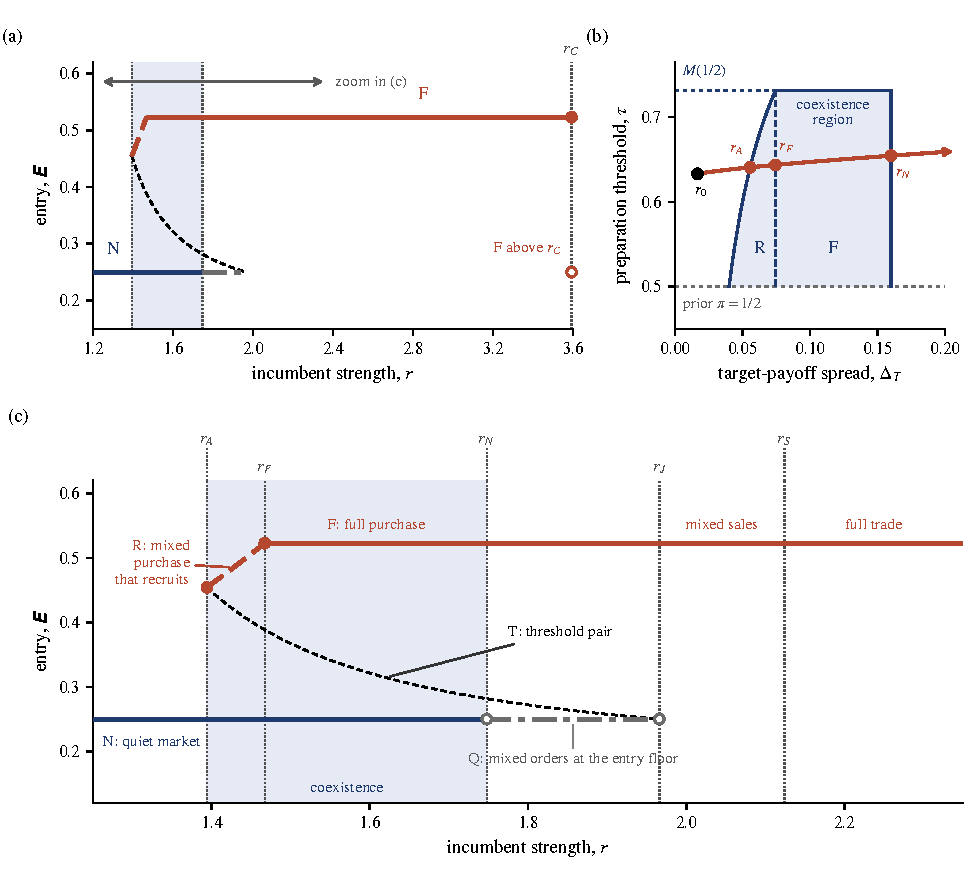
\includegraphics[width=0.62\linewidth]{../manuscript/figures/coexistence.pdf}
\caption{Equilibrium entry along the benchmark path \paper{Figure~2}. Blue: N. Red: R and F. Gray: Q. Dotted: T (CM beyond \(r_A\); C1 also admits the endpoint \(r_A\)).}\label{fig:08-coexistence}
\end{figure}

\begin{panelnote}[What changed from the Laplace version]
The Laplace version certified three isolated strengths (\reg{str_r155}, \reg{str_r160}, \reg{str_r165}), and the equilibrium correspondence between
them was unknown. In the slot version the whole equilibrium set is known along the path, each order rate has an explicit formula,
and the high class mixes over orders, not over order sizes.
\end{panelnote}

\subsection{Other priors}\label{sec:08_coexistence-priors}

Fix the investor rule IM here. For a prior \(\pi\), let \(r_N(\pi)=\mathfrak r\bigl(k/(\rho\max\{\pi,1-\pi\})\bigr)\) be the end of no trade; \(r_C(\pi)\) the
largest strength on the path with \(\tau(r)\le M(\pi)\); and define \(r_\pi\) by \(\tau(r_\pi)=\pi\) when \(\pi\in[\tau(r_0),\tau(r_2)]\). Three priors divide
the cases: \(\pi_A^{\rm lo}\) solves \(M(\pi)=\tau_A\); \(\pi_A^{\rm hi}=\tau_A\); and \(\pi_{\max}=\tau(r_*)\), where \(r_*\)
solves \(\rho\DT(r)\tau(r)=k\). From the odds of \(M(\pi)\),
\[
\pi_A^{\rm lo}=\frac{\tau_A}{\tau_A+(1-\tau_A)(1+u)}=\reg{piA_lo_B},\qquad \pi_A^{\rm hi}=\reg{piA_hi},\qquad
\pi_{\max}=\reg{pimax}\ (r_*=\reg{rstar}).
\]

\begin{resultbox}[Coexistence at every prior \paper{Cor.~A.2}]
The strengths on the path at which no informed trade and an informative equilibrium coexist are
\[
C(\pi)=\bigl\{r\in[r_0,r_2]:\ r\ge r_A,\ \ \pi<\tau(r)\le M(\pi),\ \ \rho\DT(r)\max\{\pi,1-\pi\}\le k\bigr\}.
\]
(a) Empty if \(\pi<\pi_A^{\rm lo}\); \(\{r_A\}\) at \(\pi=\pi_A^{\rm lo}\). (b) \([r_A,\min\{r_N(\pi),r_C(\pi)\}]\) if
\(\pi_A^{\rm lo}<\pi<\pi_A^{\rm hi}\): the start is \(r_A\) for every such prior and every slot. (c)
\((r_\pi,\min\{r_N(\pi),r_C(\pi)\}]\) if \(\pi_A^{\rm hi}\le\pi<\pi_{\max}\). (d) Empty if \(\pi\ge\pi_{\max}\). Entry on the
informative branch is \(\rho+(1-\rho)\min\{(1-\pi)\,b\DT(r)/k,\ b+\pi\lambda\}\).
\end{resultbox}

\paragraph{Where each condition comes from.}
\begin{itemize}[leftmargin=2em]
\item \(\rho\DT\max\{\pi,1-\pi\}\le k\): no trade survives. Against an uninformative price, a purchase earns
\(\rho\DT(1-\pi)\) and a sale earns \(\rho\DT\pi\).
\item \(\tau(r)\le M(\pi)\): with no trade alive the low class abstains, so the informative equilibrium has \(s>0\). Q is
impossible, because \(\rho\DT[1-\mu_+(s)]<\rho\DT(1-\pi)\le k\). So the purchase must reach \(\tau\).
\item \(r\ge r_A\): a purchase that recruits earns at most \(\DT(1-\tau)=J\), so \(J\ge k\).
\item \(\pi<\tau(r)\): if \(\pi\ge\tau\), no trade gives entry one after every order under C1, and it survives only if
\(\DT\max\{\pi,1-\pi\}\le k\). Then a purchase earns \(\DT[1-\mu_+(s)]<\DT(1-\pi)\le k\) and a sale earns less than
\(\DT\pi\le k\): no informative equilibrium coexists.
\end{itemize}
Two facts close the cases. \(r_A<r_N(\pi)\) for every prior, because
\(\rho\DT(r_A)\max\{\pi,1-\pi\}<\rho\DT(r_A)=\rho k/(1-\tau_A)<k\) when \(\tau_A<3/4=1-\rho\) (slack
\reg{margin_tauA_3q_B}). For \(\pi>1/2\), \(r_\pi<r_N(\pi)\iff\rho\DT(r_\pi)\tau(r_\pi)<k\iff r_\pi<r_*\iff\pi<\pi_{\max}\).
Entry: \(\Pr(X=1)=b+\pi s\); on R, \(\DT(1-\pi)b/(b+\pi s)=k\) gives \(b+\pi s=(1-\pi)b\DT/k\); on F it is \(b+\pi\lambda\).

\emph{Examples.} At \(\pi=0.45\), coexistence ends near \(1.704\).
At \(\pi=3/5\), it ends exactly at \(5/3\).
At \(\pi=0.645\), the endpoints are near \(1.504\) and \(1.637\).
At priors \(3/10\) and \(0.66\), the set is empty. % verify/08_coexistence.py

\subsection{Other tie rules}\label{sec:08_coexistence-ties}

Two alternatives show which conclusions depend on the default rules.
\begin{itemize}[leftmargin=2em]
\item Rule I0: an investor indifferent between abstention and a nonzero order abstains.
\item Rule CM: an indifferent high-cost challenger may prepare with any probability.
\end{itemize}
\begin{center}\small
\begin{tabular}{@{}lllll@{}}
\toprule
Result (prior \(1/2\)) & IM, C1 & IM, CM & I0, C1 & I0, CM\\
\midrule
Proposition~2 & holds & holds & holds & holds\\
No informed trade N & \([r_0,r_N]\) & \([r_0,r_N]\) & \([r_0,r_N]\) & \([r_0,r_N]\)\\
Mixed purchase R & \((r_A,r_F)\) & \((r_A,r_F)\) & none & none\\
Threshold pair T & \(r_A\) only & \([r_A,r_J]\) & none & none\\
Full purchase F & \([r_F,r_2]\) & \([r_F,r_2]\) & \((r_F,r_N]\cup(r_S,r_2]\) & \((r_F,r_N]\cup(r_S,r_2]\)\\
Set on \((r_N,r_J)\) & F; Q & F; Q; T & empty & empty\\
Set on \([r_J,r_S]\) & F & F (and T at \(r_J\)) & empty & empty\\
Entry after a purchase at \(r_C\) & \(1\) & any in \([\rho,1]\) & \(1\) & any in \([\rho,1]\)\\
Coexistence & \([r_A,r_N]\) & \([r_A,r_N]\) & \((r_F,r_N]\) & \((r_F,r_N]\)\\
\bottomrule
\end{tabular}
\end{center}

\paragraph{Why I0 empties \((r_N,r_S]\).} There \(\rho\DT m\le k<\rho\DT/2\), so no sale rate satisfies I0.
At abstention, a sale earns \(\rho\DT/2>k\).
A full sale earns at most \(k\), so I0 selects abstention instead.
I0 also excludes an interior mixture. At \(r=2\), for example, \(\rho\DT/2=0.03125\) and \(\rho\DT m=0.016809\).
% verify/08_coexistence.py
So IM is the investor rule under which an equilibrium exists along the whole path. The strict rise of entry along R also
needs IM, because R is a mixture at indifference.

\paragraph{What CM adds at other priors.} With investor rule IM, CM can add one strength to \(C(\pi)\): the point \(r_\pi\), where the prior equals
\(\tau\). CM lets no trade keep entry \(\rho\) when \(\rho\DT\max\{\pi,1-\pi\}\le k\).
An informative purchase at that strength needs \(J(r_\pi)>k\), or \(r_A<r_\pi\).
Both conditions hold exactly
when \(\tau_A<\pi\le\pi_{\max}\). At \(\pi_{\max}\) the point \(r_*=\reg{rstar}\) is the whole set: \(M(\pi_{\max})=\reg{M_pimax_B}\),
the zero-order posterior is \reg{mu0_pimax_B}, the full purchase earns \(\DT(r_*)[1-M(\pi_{\max})]-k=\reg{margin_cmend_B}\),
and entry is \(\rho+(1-\rho)(b+\pi_{\max}\lambda)=\reg{entry_cmend_B}\).

The tie rules matter only for the intermediate strengths: every comparison in the proof of Proposition~2 is strict
(\Cref{sec:06_main_result}).

\subsection{How the proof works}\label{sec:08_coexistence-proof}

Most of the proof is algebra: the two class lemmas, the product structure and the conditions for each form. Two monotonicity steps use exact Sturm counts.

\paragraph{The path lemma \paper{Lemma~A.4}.} (a) \(\tau\) rises on \([r_0,r_2]\): by the derivative in \Cref{sec:03_auction-derivatives}. (b) \(J\) rises on \([r_0,r_2]\): exact Sturm count. (c)
\(\DT(1-\tau)^2\) rises on \([r_0,2]\): exact Sturm count. (d) \(\DT\tau\) rises on \([r_0,r_2]\): by hand, as both
positive factors rise.

\paragraph{From a derivative to a polynomial.} Each function in (b) and (c) is a ratio \(N/D\) with \(D>0\) on the path.
Its derivative is \((N'D-ND')/D^2\), so its sign is the sign of the polynomial \(N'D-ND'\). For \(J\),
\(N=(r-1)^2(8r-r^2-\tfrac14)\) and \(D=2r(20r-r^2-1)\); in lowest integer terms
\[
Q_J(r)=4r^6-160r^5+743r^4-12r^3-614r^2+40r-1 .
\]
For \(\DT(1-\tau)^2\), \(N=(r-1)^2(8r-r^2-\tfrac14)^2\) and \(D=2r(20r-r^2-1)^2\), which give the degree-10 polynomial
\(16r^{10}-1280r^9+29256r^8-229344r^7+562917r^6-32808r^5-374607r^4+48456r^3-2685r^2+80r-1\).

\paragraph{Exact Sturm counts.} Sturm's theorem counts the distinct real roots of a polynomial \(P\) in \((a,b]\) with no
approximation. Build \(p_0=P\), \(p_1=P'\), \(p_{i+1}=-\operatorname{rem}(p_{i-1},p_i)\) until the remainder is zero. Delete zero values at \(x\).
Let \(V(x)\) count the sign changes in the remaining sequence. The number of distinct roots in \((a,b]\) is
\(V(a)-V(b)\). With rational coefficients and rational end points, every step is exact rational arithmetic. A count of
zero plus a positive value at one point proves that the polynomial is positive on the whole interval.

\paragraph{Rational root brackets.} \(r_A\), \(r_J\) and \(r_*\) are roots of strictly monotone rational functions.
Each function has an exact sign at a rational point.
Bisection retains endpoints with opposite signs, so the bracket contains the unique root. Thresholds that depend on \(\eu\) use rational bounds on
\(\eu\) from its series. A separate scan rebuilds the set from the flow law at 241 strengths for the four pairs of tie
rules; it is a cross-check and enters no proof step.

\begin{panelnote}[How to say it, and our check]
``Proposition~3 is algebra, except two monotonicity facts. Each is the sign of an integer polynomial on a rational
interval, and an exact Sturm count settles it.'' Our script \texttt{verify/08\_coexistence.py} builds \(N'D-ND'\) for both
functions from the primitives with exact fractions and reproduces both polynomials coefficient by coefficient. Its Sturm
count gives zero roots of \(Q_J\) in \((r_0,r_2]\) and zero roots of the degree-10 polynomial in \((r_0,2]\); both are
positive at \(r_0\) (\(Q_J(r_0)=\reg{QJ_r0}\)).
\end{panelnote}
